% !TeX spellcheck = en_US
\documentclass[french]{yLectureNote}

\title{Mécanique}
\subtitle{Mécanique du point}
\author{Paulhenry Saux}
\date{\today}
\yLanguage{Français}

\professor{S.Deheuvels}%sebastien.deveuhels.irap.omp.eu

\usepackage{graphicx}%----pour mettre des images
\usepackage[utf8]{inputenc}%---encodage
\usepackage{geometry}%---pour modifier les tailles et mettre a4paper
%\usepackage{awesomebox}%---pour les boites d'exercices, de pbq et de croquis ---d\'esactiv\'e pour les TP de PC
\usepackage{tikz}%---pour deiffner + d\'ependance de chemfig
\usepackage{tkz-tab}
\usepackage{chemfig}%---pour deiffner formules chimiques
\usepackage{chemformula}%---pour les formules chimiques en \'equation : \ch{...}
\usepackage{tabularx}%---pour dimensionner automatiquement les tableaux avec variable X
\usepackage{awesomebox}%---Pour les boites info, danger et autres
\usepackage{menukeys}%---Pour deiffner les touches de Calculatrice
\usepackage{fancyhdr}%---pour les en-t\^ete personnalis\'ees
\usepackage{blindtext}%---pour les liens
\usepackage{hyperref}%---pour les liens (\`a mettre en dernier)
\usepackage{caption}%---pour la francisation de la l\'egende table vers Tableau
\usepackage{pifont}
\usepackage{array}%---pour les tableaux
\usepackage{lipsum}
\usepackage{yFlatTable}
\usepackage{multicol}
\newcommand{\Lim}[1]{\lim\limits_{\substack{#1}}\:}
\renewcommand{\vec}{\overrightarrow}
\newcommand{\norm}[1]{||\vec{#1}||}
\DeclareMathOperator\arctanh{arctanh}
\begin{document}

%\titleOne
\setcounter{chapter}{3}
	\chapter{Mouvements circulaires et systèmes de coordonnées }
\section{Coordonnées polaires}
Il s'agit d'un système de coordonnées qui permet de repérer l'espace à 2 dimensions.
\subsection{Base polaire}
% \begin{multicols}{2}
% \columnbreak
% \end{multicols}
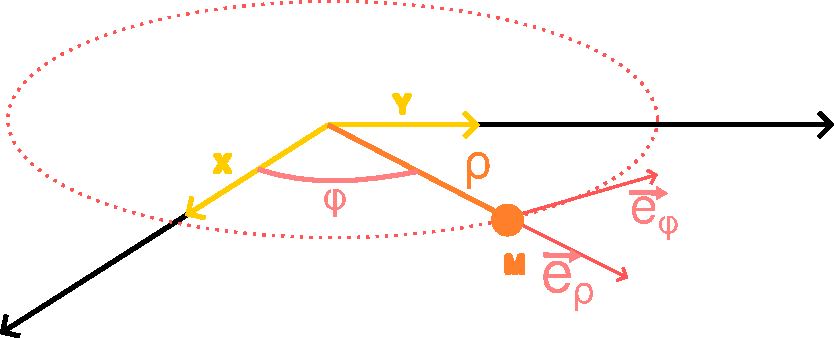
\includegraphics[scale=0.5]{base_p}

On introduit une base dite locale (elle dépend du point où l'on se trouve. On définit
\begin{itemize}
 \item $\vec{e_{\rho}}$, unitaire dans la direction de $\vec{OM}$. Ainsi, $\vec{e_{\rho}} = \frac{\vec{OM}}{\norm{OM}}$
 \item $\rho = \norm{OM} >0$
 \item $\varphi = (\vec{e_x},\vec{e_{\rho}})$
 \item $\vec{e_{\varphi}}$ orthogonal à $\vec{e_{\rho}}$ et dans le sens de l'angle $\varphi$\marginCritical{Il est toujours dirigé dans le sens trigonométrique, m\^eme si $\varphi$ est négatif !}
\end{itemize}
Cette base dépend du point où l'on se trouve. La position de chaque point est définie par $\rho$ et $\varphi$.
\subsubsection{Relation entre base polaire et cartésienne}
\begin{itemize}
 \item $\vec{e_{\rho}} = \cos (\varphi) \vec{e_x}+\sin (\varphi) \vec{e_y}$
 \item $\vec{e_{\varphi}} = -\sin( \varphi) \vec{e_x}+\cos( \varphi) \vec{e_y}$
\end{itemize}
\subsection{Vecteur position}
$\vec{OM} = \rho \vec{e_{\rho}}$\marginCritical{Il n'y a pas de composantes selon $\vec{e_{\varphi}}$.}
\subsection{Vecteur vitesse}
\begin{multicols}{2}
\begin{flalign*}
\vec{v} &= \frac{d\vec{OM}}{dt}\\
&= \frac{d}{dt}(\rho \vec{e_{\rho}})\\
&= \frac{d\rho}{dt}\vec{e_{\rho}}+\rho \frac{d\vec{e_{\rho}}}{dt}
\end{flalign*}
\columnbreak
\begin{flalign*}
\frac{d\vec{e_{\rho}}}{dt} &= \frac{d}{dt}(\cos\varphi \vec{e_x} + \sin \varphi \vec{e_y})\\
&= -\frac{d\varphi}{dt}\sin\varphi \vec{e_x}+\frac{d\varphi}{dt}\cos\varphi \vec{e_y}\\
&= \frac{d\varphi}{dt}(-\sin\varphi\vec{e_x}+\cos\varphi\vec{e_y})\\
&= \dot{\varphi}(-\sin\varphi\vec{e_x}+\cos\varphi\vec{e_y})\\
&= \dot{\varphi}(\vec{e_{\varphi}})
\end{flalign*}
\end{multicols}
\begin{theorem}[Vitesse en coordonnées polaire]
$\vec{v} = \dot{\rho}\vec{e_{\rho}}+\rho\dot{\varphi}\vec{e_{\varphi}}$
\end{theorem}


\subsection{Vecteur accélération en polaire}
\subsubsection{Calcul de la dérivé du vecteur $\varphi$}
\begin{flalign*}
\frac{d\vec{e_{\varphi}}}{dt} &= \frac{d}{dt}(-\sin( \varphi) \vec{e_x}+\cos( \varphi) \vec{e_y})\\
&= -\cos(\varphi)\times\frac{d\varphi}{dt}\vec{e_x} - \sin(\varphi)\frac{d\varphi}{dt}\vec{e_y}\\
&= -\dot{\varphi}(\cos(\varphi)\vec{e_x}+\sin(\varphi)\vec{e_y})\\
&= -\dot{\varphi}\vec{e_{\rho}}
\end{flalign*}
On dérive $\vec{v}$\marginTips{Pour dériver $\rho\dot{\varphi}\vec{e_{\varphi}}$, on va utiliser la formule $(uvw)' = u'vw+uv'w+uvw'$
}
\begin{flalign*}
\frac{d\vec{v}}{dt} &= \frac{d}{dt}({\color{orange}\dot{\rho}\vec{e_{\rho}}} + {\color{red}\rho\dot{\varphi}\vec{e_{\varphi}}})\\
&= {\color{orange}\ddot{\rho}\vec{e_{\rho}} + \dot{\rho} \frac{d\vec{e_{\rho}}}{dt}} + {\color{red}\dot{\rho}\dot{\varphi}\vec{e_{\varphi}}+\rho\ddot{\varphi}\vec{e_{\varphi}} + \rho\dot{\varphi}\frac{d\vec{e_{\varphi}}}{dt}}\\
&= {\color{orange}\ddot{\rho}}\vec{e_{\rho}} + {\color{red}\dot{\rho} \dot{\varphi}}(\vec{e_{\varphi}}) +{\color{red}\dot{\rho} \dot{\varphi}}\vec{e_{\varphi}}+{\color{purple}\rho\ddot{\varphi}}\vec{e_{\varphi}} + \rho\dot{\varphi} (-\dot{\varphi})\vec{e_{\rho}}\\
&= ({\color{orange}\ddot{\rho}}-\rho\dot{\varphi}^2)\vec{e_{\rho}}+({\color{purple}\rho\ddot{\varphi}}+2{\color{red}\dot{\rho} \dot{\varphi}})\vec{e_{\varphi}}\\
\end{flalign*}
\begin{theorem}[accélération en coordonnées polaire]
\[\vec{a} =  (\ddot{\rho}-\rho\dot{\varphi}^2)\vec{e_{\rho}}+(\rho\ddot{\varphi}+2\dot{\rho}\dot{\varphi})\vec{e_{\varphi}}\]
\end{theorem}
\subsection{Cas particulier du mouvement circulaire}
La distance du point $M$ à un point $O$, choisi comme l'origine du repère, reste constante au cours du temps. Dans la base polaire, on a
\begin{itemize}
 \item $\rho(t) = R = $ Constante.
 \item $\dot{\rho}(t) = 0$ car la dérivée d'une constante est nulle.
\end{itemize}


\subsubsection{Expression des vecteurs}
$\vec{OM} = \rho \vec{e_{\rho}} = R \vec{e_{\rho}}$

$\displaystyle \vec{v} = R\frac{d\vec{e_{\rho}}}{dt} = R\dot{\varphi}\vec{e_{\varphi}}$\marginInfo{On retrouve le m\^eme résultat en partant de l'expression générale : $\vec{v} =  \dot{\rho}\vec{e_{\rho}}+\rho\dot{\varphi}\vec{e_{\varphi}} = R\dot{\varphi}\vec{e_{\varphi}}$}

$\displaystyle \vec{a} = \frac{d}{dt}(R\dot{\varphi}\vec{e_{\varphi}}) = R\ddot{\varphi}\vec{e_{\varphi}}+R\dot{\varphi}\frac{\vec{e_{\varphi}}}{dt} = R \ddot{\varphi}\vec{e_{\varphi}} - R\dot{\varphi}^2\vec{e_{\rho}}$. \marginInfo{On la retrouve à partir de l'expression de l'accélération en polaire. En effet, les termes avec la dérivée première ou seconde s'annulent.}


\subsubsection{Exemple du pendule}

\includegraphics[scale=0.5]{pendule}

On étudie le mouvement de la masse $M$ de masse $m$ attachée au bout d'un fil de longueur $l$.

On a $\norm{OM} = l =$  qui est constante. On a donc un mouvement circulaire.

Le système est la masselotte, avec un référentiel terrestre muni de la base polaire.

On fait le bilan des forces : $\sum \vec{F} = \vec{P}+\vec{T}$.

On projette dans la base : $\vec{T} = -T\vec{e_{\rho}}$ et $\vec{P} =mg\cos(\varphi)\vec{e_{\rho}}-mg\sin(\varphi)\vec{e_{\varphi}} $

On dérive 2 fois pour trouver l'accélération : $\vec{OM} = l\vec{e_{\varphi}}, \vec{v} = l\dot{\varphi}\vec{e_{\varphi}}, \vec{a} = -l\dot{\varphi}^2\vec{e_{\rho}} + l\ddot{\varphi}\vec{e_{\varphi}}$.
En appliquant le PFD, on obtient 2 équations scalaires :
\[\left\{\begin{matrix}
m(-l\dot{\varphi}^2) &= mg\cos(\varphi) - T\\
m(l\ddot{\varphi}) &= -mg\sin(\varphi) + 0
\end{matrix}\right.
\]


On utilise l'équation 2, sans $T$ à l'intérieur : $ml\ddot{\varphi} = -mg\sin(\varphi)$ et $l\ddot{\varphi} = -g\sin(\varphi)$

On a une équation de la forme $l\ddot{\varphi} + g\sin(\varphi) = 0$ et $\ddot{\varphi} + \frac{g}{l}\sin(\varphi) = 0$ Il s'agit d'une équation différentielle du second degré homogène, mais non linéaire.

\subsection{Cas du mouvement circulaire uniforme}
\subsubsection{Pulsation}
La vitesse $V$ est constante, tout comme $\norm{OM} = R$.

 La vitesse vaut $R\dot{\varphi}\vec{e_{\varphi}}$ et $\norm{v} = V = R|\dot{\varphi}|$.

 Donc $|\dot{\varphi}| = \frac{V}{R}$.

Dans ce cas, la vitesse angulaire $\dot{\varphi}$ est constante et on l'appelle la pulsation, notée $\Omega$ ou $\omega$. Elle se mesure en rad$\cdot$s$^{-1}$.\marginCritical{On l'écrit avec $\omega$ que quand elle est constante. }

On suppose que $\varphi(t)$ est orienté de sorte que $\dot{\varphi} >0$. Dans ce as, $|\dot{\varphi}| = \dot{\varphi} = \frac{V}{R}$.
\subsubsection{Expression des vecteurs}

On obtient :
$\vec{v} = V\vec{e_{\varphi}} = R\omega \vec{e_{\varphi}}$ et

$\vec{a} = -R\dot{\varphi}^2\vec{e_{\rho}} + R\ddot{\varphi}\vec{e_{\varphi}} = -R\omega^2\vec{e_{\rho}} = -R\frac{V^2}{R^2}\vec{e_{\rho}} = -\frac{V^2}{R}\vec{e_{\rho}}$.

%Résumé : $\vec{v} = R\omega \vec{e_{\varphi}}$ et $\vec{a} = \frac{-V^2}{R} \vec{e_{\rho}}$.

\subsubsection{Nouveaux éléments de description}
\begin{itemize}
 \item La pulsation $\omega$ = nombre de radians parcourus par secondes (constante)
 \item La période $T$ = Temps  nécessaire pour faire un tour : $T = \frac{2\pi}{\omega}$ On peut retrouver cette relation avec $v=d/t$.
 \item La fréquence : Nombre de tours éffectués par seconde : $\nu = \frac{1}{T}$.
\end{itemize}
\subsection{Exemple : Orbite de la Terre autour du Soleil}

Hypothèse : Trajectoire circulaire.

Schéma 4.1.6.1

On obtient ces expressions :

$\vec{ST} = R\vec{e_{\rho}}$,

$\vec{v} = R\dot{\varphi}\vec{e_{\varphi}}$

$\vec{a} = -R\dot{\varphi}^2\vec{e_{\rho}} + R\ddot{\varphi}\vec{e_{\varphi}}$

On fait le bilan des forces : $\vec{F_g} = -G\frac{m_sm_t}{d^2}\vec{e_{\rho}}$.

On applique le PFD : $m_T\vec{a} = \vec{F_g}$.

Donc on obtient 2 équations scalaires :
\[\left\{\begin{matrix}
-R\dot{\varphi}^2 &= -G\frac{m_s}{d^2} \iff R\dot{\varphi}^2 &= G\frac{m_s}{d^2}\\
R\ddot{\varphi} &= 0
\end{matrix}\right.
\]

On remarque que $\ddot{\varphi} = 0$, donc $\dot{\varphi}$ est constant et on le not alors $\omega$.

Donc $\vec{v} = R\dot{\varphi}\vec{e_{\varphi}} = R\omega\vec{e_{\varphi}}$.

De plus, $R\omega^2 = \frac{Gm_s}{R^2} \iff \omega = \sqrt{\frac{GM_s}{R^3}}$.

On peut en déduire :
\begin{itemize}
 \item La vitesse de la terre sur son orbite : $v = R\omega = R \times \sqrt{\frac{GM_s}{R^3}} = \sqrt{\frac{GM_s}{R}}$
 \item La période de la terre sur son orbite : $T = \frac{2\pi}{\omega} = 2\pi \sqrt{R^3}{GM_s}$.
\end{itemize}


Période de la terre sur son orbite : $T = \frac{2\pi}{\omega} = \frac{2\pi}{\sqrt{\frac{GM_s}{R^3}}}$.

On est dans un cas particulier de la troisème loi de Kepler : $T^2/R^3 = 4\pi^2\times \frac{R^3}{GM_s}\times \frac{1}{R^3} = \frac{4\pi^2}{GM_s}$.
\section{Coordonnées cylindriques}
C'est un système de coordonnées permettant de repérer l'espace à 3 dimensions. Le principe : On construit la base cylindrique avec
\begin{itemize}
 \item Une base polaire du type $(\vec{e_{\rho}},\vec{e_{\varphi}})$
 \item Un vecteur unitaire $\vec{e_z} $ orthogonal à $ (\vec{e_{\rho}},\vec{e_{\phi}})$ orienté tel que $ (\vec{e_{\rho}},\vec{e_{\varphi}}, \vec{e_z})$ soit une BOND. le vecteur unitaire $\vec{e_z}$ reste fixe au cours du temps.
\end{itemize}
\begin{multicols}{2}
\begin{itemize}
 \item $\rho(t) = OH$
 \item $\varphi(t) = (\vec{e_x},\vec{OH})$
 \item $\vec{OM} = \rho\vec{e_{\rho}} + z\vec{e_z}$.
\end{itemize}
Lien entre les cordonnées :
\begin{itemize}
 \item $\rho = \sqrt{x^+y^2}$
 \item $\tan \varphi = \frac{y}{x}$
 \item $z=z$
 \item $x=\rho\cos(\varphi)$
 \item $y= \rho\sin(\varphi)$
\end{itemize}
\columnbreak
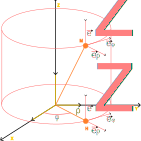
\includegraphics[scale=0.5]{base_c}


\end{multicols}



\subsubsection{Expression des vecteurs}
La vitesse : $\vec{v} = \frac{d}{dt}(\rho\vec{e_{\rho}} + z\vec{e_z}) = \dot{\rho}\vec{e_{\rho}} + \rho\dot{\varphi}\vec{e_{\varphi}} + z\vec{e_z}$

L'accélération : $\vec{a} = (\ddot{\rho}-\rho\dot{\varphi}^2)\vec{e_{\rho}} + (\rho\ddot{\varphi}+2\dot{\rho}\dot{\varphi})\vec{e_{\varphi}} + \ddot{z}\vec{e_z}$ C'est comme l'accélération en polaire mais on rajoute les cordonnées en $z$.
\section{Coordonnées sphériques}
C'est aussi un système de coordonnées pour repérer l'espace à troid dimensions.

Base :$\vec{e_r},\vec{e_{\theta}},\vec{e_{\varphi}}$
\subsection{Construction}
On construit $\vec{e_r}$, vecteur unitaire dans la direction et sens de $\vec{OM}$. On a $\vec{e_r} = \frac{\vec{OM}}{\norm{OM}}$. On a lors $\vec{OM} = r \vec{e_r}$

On introduit le point $H$, projeté orthogonal de $M$ sur le plan $(Oxy)$ et la base polaire associée à H.

On introduit l'angle $\theta$ entre $\vec{e_z}$ et $\vec{e_r}$ et le vecteur unitaire $\vec{e_{\theta}}$ orthogonal à $\vec{e_r}$

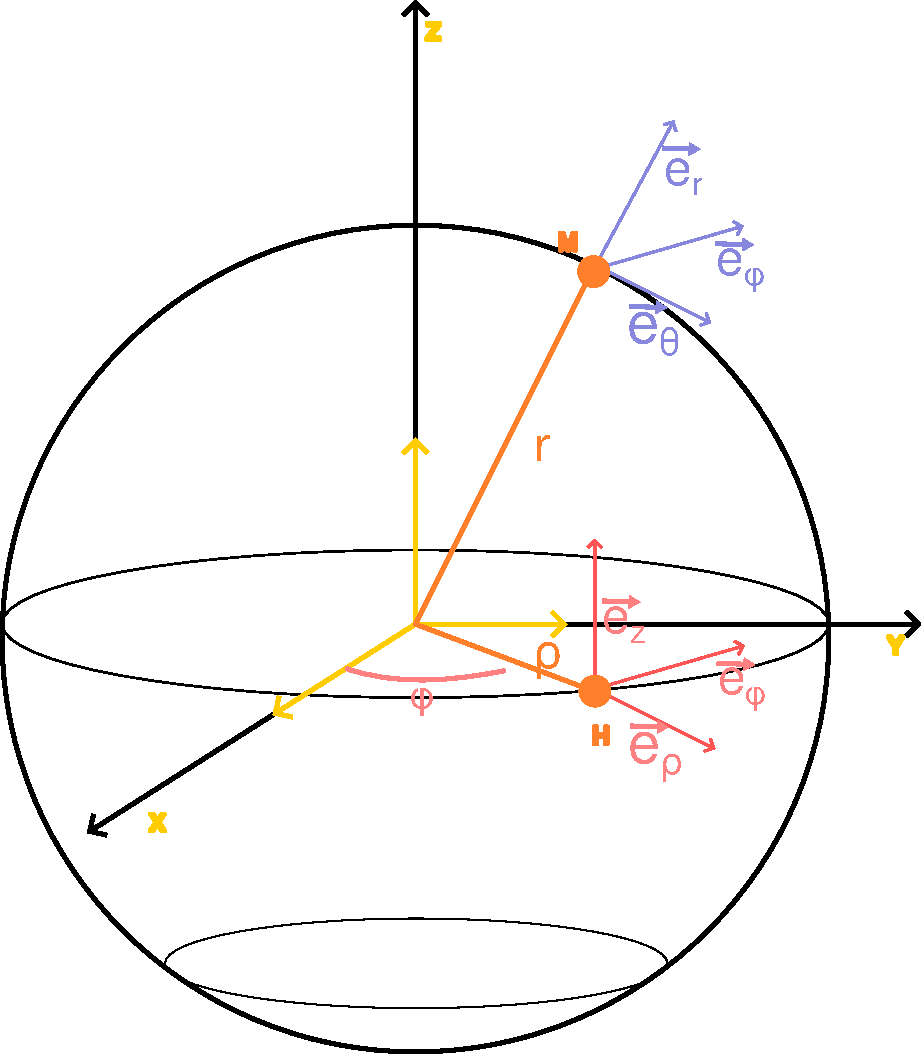
\includegraphics[scale=0.5]{base_s}

Les vecteurs $\vec{e_r},\vec{e_{\theta}},\vec{e_{\varphi}}$ sont orthogonaux entre eux et unitaires, donc forment une BOND.

Dans ce système de coordonnées, un point $M$ est repéré par 3 grandeurs : $r,\theta,\varphi$.

$x= \rho \cos(\varphi) = r\sin\theta \cos\varphi$

$y = \rho \sin(\varphi) = r\sin\theta \sin\varphi$

$z = r \cos(\varphi) = r\cos\theta$

$ \rho = r\sin(\varphi)$

$r = \sqrt{x^2+y^2+z^2}$

$\theta = \sin^{-1} \frac{\rho}{r}$
\subsection{Vecteurs}
vecteur position : $\vec{OM} = r\vec{e_r}$

vecteur vitesse : $\vec{v} = \dot{r}\vec{e_r}+r\dot{\theta}\vec{e_{\theta}}+r\sin\theta \dot{\varphi}\vec{e_{\varphi}}$.
\section{Déplacement élémentaire}
$\vec{M(t)M(t+\mathrm{d}t} = \mathrm{d}\vec{OM} = \vec{v}\times \mathrm{d}t = (\frac{\mathrm{d}x}{\mathrm{d}t}\vec{e_x} + \frac{\mathrm{d}y}{\mathrm{d}t}\vec{e_y} + \frac{\mathrm{d}z}{\mathrm{d}t}\vec{e_z})$

En coordonnées cylindriques :

$\mathrm{d} \vec{OM} = (\frac{\mathrm{d}\rho}{\mathrm{d}t}\vec{e_{\rho}} + \frac{\mathrm{d}\varphi}{\mathrm{d}t}\vec{e_{\varphi}} + \frac{\mathrm{d}z}{\mathrm{d}t}\vec{e_z})$

En coordonnées sphériques : $\mathrm{d} \vec{OM} = \mathrm{d}r \vec{e_r} + r\mathrm{d}\theta \vec{e_{\theta}} + r\sin\theta \mathrm{d}\varphi \vec{e_{\varphi}}$

\section{Base de Frenet}
Base de l'espace en 2D. On introduit :
\begin{itemize}
 \item $\vec{e_t}$, unitaire et tangent à la trajectoire et dans le sens du mouvement : $\frac{\vec{v}}{\norm{v}}$
 \item $\vec{e_n}$, orthogonal à $\vec{e_t}$. Il est dirigé vers l'intérieur de la concavité.
 \item On peut ajouter un troisème vecteur $\vec{e_b}$ tel que les 3 forment une BOND
\end{itemize}
Vecteur vitesse : $\vec{v} = v\vec{e_t}$

Vecteur accélération : $\vec{a} = \frac{\mathrm{d}}{\mathrm{d}t} + \frac{v^2}{R}\vec{e_r}$, avec $R$ le rayon de courbure

Rmq : Pour un mouvement circulaire, dans la base polaire et de frenet, le vecteur $\vec{e_r}$ est opposé à $\vec{e_{\rho}}$.

\end{document}

